\documentclass[12pt]{article}

\usepackage[letterpaper, hmargin=0.75in, vmargin=0.75in]{geometry}
\usepackage{float}
\usepackage{hyperref}
\usepackage{graphicx}
\usepackage{url}
\usepackage{copyrightbox}
\usepackage{listings}
\usepackage{csvsimple}
\usepackage{listings}
\usepackage{amsmath}



\pagestyle{empty}

\title{ECE 495: Autonomous Vehicles\\Final Exam}
\author{Zahin Mohammad}
\date{\today}

\begin{document}

\maketitle
\section{Question 1}
The level of automation of the ADS that operates the taxi is level 4.
\section{Question 2}
\subsection{a}
\begin{align*}
    = \begin{bmatrix}
        -4 & 6 & 3 & 2 \\
    \end{bmatrix} \\
\end{align*}
\subsection{b}
The resulting image would be shifted down and to the left by one pixel.
\subsection{c}
I would address the problem by converting the image to HSV and look at the hue plane to select the stop sign.
\subsection{d}
The step applying non-maximum suppression suppresses pixels with non-maximum gradient, resulting in thin edges.
\subsection{e}
The gradient applied is:
\begin{equation*}
    \frac{\partial{f}}{\partial{x}}
\end{equation*}
This is because it is highlighting changes in intensity along the $x$ direction.
This can be seen because vertical lines are highlighted clearly (the stem).
\subsection{f}
In the hough space using polar coordinates, the pixel would correspond to a single sinusoid.

\section{Question 3}
\subsection{a}
\begin{align*}
    P(y|x;w_1, w_0, \sigma) = N(w_1*x + w_0, \sigma)
\end{align*}

\subsection{b}
\begin{align*}
    (0.3-0.5)^2 = 0.04
\end{align*}

\subsection{c}
\begin{align*}
    -ln(0.6) = 0.51
\end{align*}

\subsection{d}

$Relu(W_1*x + b_1$):
\begin{align*}
    = \begin{bmatrix}
        2 \\
        1 \\
        3 \\
    \end{bmatrix} \\
\end{align*}

$W_2*Relu(W_1*x+b_1)+b_2$:
\begin{align*}
    = \begin{bmatrix}
        2  \\
        19 \\
        20 \\
    \end{bmatrix} \\
\end{align*}

$Softmax(W_2*Relu(W_1*x+b_1)+b_2)$:
\begin{align*}
    = \begin{bmatrix}
        0.000 \\
        0.269 \\
        0.731 \\
    \end{bmatrix} \\
\end{align*}
Therefore the inference probability for the correct class is 73.1\%.

\subsection{e}
\begin{figure}[H]
    \centering
    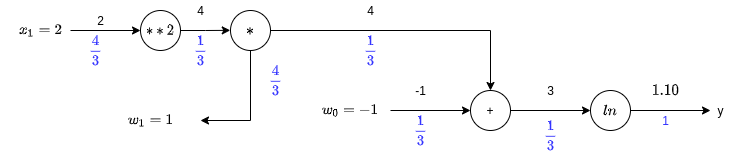
\includegraphics[width=0.6\linewidth]{3e.png}
    \caption{Back propagation}
\end{figure}

\subsection{f}
Overfitting is when the training loss is low and the validation and testing loss is high.

\subsection{g}
This is called regularization. Regularization puts a cost on more complex models, i.e. it creates a preference for simpler models.

\section{Question 4}
\subsection{a}
Intersection: $4500-500=4000$\\
Union: $7500+500=8000$\\
IoU: $\frac{4000}{8000}=\frac{1}{2}$

\subsection{b}
Pixel Accuracy:
\begin{align*}
     & = \frac{\#TP + \#TN}{\#TP + \#TN + \#FP + \#FN} \\
     & = \frac{4000+(100000-7500-500)}{100000}         \\
     & = 96\%
\end{align*}

The pixel accuracy is high because the class representation is small compared to the entire set of pixels, therefore it is easy to achieve high pixel accuracy by classifying a majority of pixels as not that class.
In contract the IoU takes the size of each class into account.

\subsection{c}
One technique that can be used to obtain detailed shape contours in the segmented image is upsampling via cubic or linear upsampling opposed to nearest neighbor. By applying upsampling, the output image reconstructs its details.

\section{Question 5}
\subsection{a}
There is one true positive ($TP=1$), which is the white car as it meets the IoU and score threshold.
There is two false positives ($FP=2$), which is the two detections in the middle. They both meet the score threshold but fail the IoU threshold.
The number of false negatives are the number of ground truths minus the true positives, therefore there is 1 false negative ($FN=1$).


\subsection{b}
There are four boxes left after non-maximal suppression. \\
The person with score of 0.3 is above threshold and is not overlapping other person classes above threshold, therefore it remains.
The car with score of 0.8 is above threshold and does not overlap any other car, therefore it remains.
The cars with score of 0.4 and 0.6 are above threshold but overlap greater then 50\% therefore only the car score of 0.6 remains.
The cyclist is above threshold and does not overlap any other cyclists therefore it remains.

\section{Question 6}
\subsection{a}
\begin{equation*}
    P(x_t | x_{t-1}, u_t) = N(A_tx_{t-1} + B_tu_tR_t)
\end{equation*}
\begin{equation*}
    P(y_t|x_t,u_t, Q_t)
\end{equation*}
\subsection{b}
Yes this model satisfies the Markov property because only the current state is needed to predict the state at the next time step.
\subsection{c}
The arrows represent conditional probability for a target node (destination of arrow), with the source nodes (origin of the arrows) being the conditions.
The single incoming arrow arrow between $C$ and $D$ represents $P(D|C)$. The double incoming arrows between $A$ and $B$ to $C$ represents $P(C|A,B)$.

\section{Question 7}
\subsection{a}
Let $W_t$ denote distribution of weather. Let the t vector represent being sunny vs overcast ($W_t=s$ vs $W_t=o$).
\begin{align*}
    P(W_t)         & = \begin{bmatrix}
        P(W_t = s) \\
        P(W_t = o) \\
    \end{bmatrix} \\
    P(W_t|W_{t-1}) & = \begin{bmatrix}
        P(W_t = s | W_{t-1} = s) & P(W_t = s | W_{t-1} = o) \\
        P(W_t = o | W_{t-1} = s) & P(W_t = o | W_{t-1} = o) \\
    \end{bmatrix} \\
    P(W_t|W_{t-1}) & = \begin{bmatrix}
        0.8 & 0.8 \\
        0.2 & 0.2 \\
    \end{bmatrix}
\end{align*}
Uninformative prior implies:
\begin{align*}
    P(W_1) & = \begin{bmatrix}
        0.5 \\
        0.5 \\
    \end{bmatrix} \\
\end{align*}
Therefore the weather distribution on day three is:
\begin{align*}
    P(W_3) & = \begin{bmatrix}
        0.8 & 0.8 \\
        0.2 & 0.2 \\
    \end{bmatrix}
    *
    \begin{bmatrix}
        0.8 & 0.8 \\
        0.2 & 0.2 \\
    \end{bmatrix}
    *
    \begin{bmatrix}
        0.5 \\
        0.5 \\
    \end{bmatrix}            \\
           & = \begin{bmatrix}
        0.8 & 0.8 \\
        0.2 & 0.2 \\
    \end{bmatrix}
    *
    \begin{bmatrix}
        0.5 \\
        0.5 \\
    \end{bmatrix}            \\
           & = \begin{bmatrix}
        0.8 \\
        0.2 \\
    \end{bmatrix}
\end{align*}
Therefore the probability of being sunny on the third day is 80\%.\\
This can be generalized for to:
\begin{align*}
    P(W_t) & = \begin{bmatrix}
        0.8 & 0.8 \\
        0.2 & 0.2 \\
    \end{bmatrix}
    *
    W_1
\end{align*}
The probability distribution the 100th day is:
\begin{align*}
    P(W_{100}) & = \begin{bmatrix}
        0.8 & 0.8 \\
        0.2 & 0.2 \\
    \end{bmatrix}
    *
    \begin{bmatrix}
        0.5 \\
        0.5 \\
    \end{bmatrix}                \\
               & =
    \begin{bmatrix}
        0.8 \\
        0.2 \\
    \end{bmatrix}                \\
\end{align*}
Therefore the probability of being sunny on the 100th day is 80\%.
\subsection{b}
\subsubsection{1}
Having log odds of zero before the measurement means there is no information for that cell.
\subsubsection{2}

\begin{figure}[H]
    \centering
    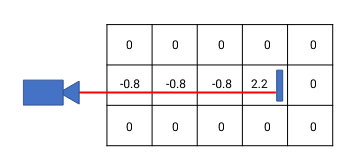
\includegraphics[width=0.6\linewidth]{7b.png}
    \caption{Occupancy Grid}
\end{figure}

\begin{align*}
    Log(O(1,2)) & = log(\frac{P}{1-P})   \\
                & = log(\frac{0.3}{0.7}) \\
                & = log(\frac{3}{7})     \\
                & \approx -0.8
\end{align*}

\begin{align*}
    Log(O(2,2)) & = log(\frac{P}{1-P})   \\
                & = log(\frac{0.3}{0.7}) \\
                & = log(\frac{3}{7})     \\
                & \approx -0.8
\end{align*}

\begin{align*}
    Log(O(3,2)) & = log(\frac{P}{1-P})   \\
                & = log(\frac{0.3}{0.7}) \\
                & = log(\frac{3}{7})     \\
                & \approx -0.8
\end{align*}

\begin{align*}
    Log(O(4,2)) & = log(\frac{P}{1-P})   \\
                & = log(\frac{0.9}{0.1}) \\
                & = log(9)               \\
                & \approx 2.2
\end{align*}

\subsection{c}
No, a square of a Gaussian-distributed variables does not yield a variable that is Gaussian distributed.
\subsection{d}
$a$ and $d$ are positive.\\
$a$ and $d$ are not equal, $d>a$.\\
The likely values of $c$ and $b$ are $a=0$, $b=0$.\\
$g$ and $f$ are equal.\\
$g$ and $f$ are negative.\\

\subsection{e}
There are three covaraince matrices involved in the calculations for a single time step in kalman filtering.
There are $R_k$, $Q_k$ and $P_k$.
\subsection{f}
\subsubsection{1}
\begin{align*}
    \begin{bmatrix}
        l_x      \\
        l_y      \\
        \psi     \\
        \dot\psi \\
        v        \\
    \end{bmatrix}_t & = \begin{bmatrix}
        l_x +  \Delta{t} * v * cos(\psi) \\
        l_y + \Delta{t}*v*sin(\psi)      \\
        \psi + \Delta{t} * \dot\psi      \\
        \dot\psi                         \\
        v                                \\
    \end{bmatrix}_{t-1}
    +
    \epsilon_t
\end{align*}
\subsubsection{2}
\begin{align*}
    f_2 & =
    \begin{bmatrix}
        l_y + \Delta{t} * v * sin(\psi) \\
    \end{bmatrix}
\end{align*}

\begin{align*}
    F_2 & = \frac{\partial{f_2}}{\partial{x}} \\
        & = \begin{bmatrix}
        \frac{\partial{f_2}}{\partial{l_x}} & \frac{\partial{f_2}}{\partial{l_y}} & \frac{\partial{f_2}}{\partial{\psi}} & \frac{\partial{f_2}}{\partial{\dot\psi}} & \frac{\partial{f_2}}{\partial{v}}
    \end{bmatrix}        \\
        & = \begin{bmatrix}
        0 & 1 & \Delta{t}*v*cos(\psi) & 0 & \Delta{t}*sin(\psi)
    \end{bmatrix}
\end{align*}
\subsubsection{3}
Process noise is additive, therefore:
\begin{align*}
    E & = I                          \\
      & = \begin{bmatrix}
        1 & 0 & 0 & 0 & 0 \\
        0 & 1 & 0 & 0 & 0 \\
        0 & 0 & 1 & 0 & 0 \\
        0 & 0 & 0 & 1 & 0 \\
        0 & 0 & 0 & 0 & 1 \\
    \end{bmatrix}
\end{align*}
\subsubsection{4}
\begin{align*}
    y_t                          & = g(x_t, \delta_t)           \\
                                 & = G*x_t + \delta_t           \\
    \begin{bmatrix}
        l_x  \\
        l_y  \\
        \psi \\
    \end{bmatrix}_t & = \begin{bmatrix}
        1 & 0 & 0 & 0 & 0 \\
        0 & 1 & 0 & 0 & 0 \\
        0 & 0 & 1 & 0 & 0 \\
    \end{bmatrix}
    *
    \begin{bmatrix}
        l_x      \\
        l_y      \\
        \psi     \\
        \dot\psi \\
        v        \\
    \end{bmatrix}_t
    +
    \delta_t
\end{align*}
\subsubsection{5}
\begin{align*}
    G & = \begin{bmatrix}
        1 & 0 & 0 & 0 & 0 \\
        0 & 1 & 0 & 0 & 0 \\
        0 & 0 & 1 & 0 & 0 \\
    \end{bmatrix}
\end{align*}
\subsubsection{6}
Measurement noise is additive, therefore:
\begin{align*}
    D & = I                          \\
      & = \begin{bmatrix}
        1 & 0 & 0 \\
        0 & 1 & 0 \\
        0 & 0 & 1 \\
    \end{bmatrix}
\end{align*}
\subsubsection{7}
\begin{align*}
    \mu_0    & = 0            \\
    {\sum}_0 & = (0.1)I_{5x5}
\end{align*}
\subsection{g}
\subsubsection{1}
The steady state kalman filter would be applicable in this alternative formulation.
\subsubsection{2}
The assumption that the $\dot\psi$ is constant (from previous question) does not hold in this question.
\subsubsection{3}
The heading rate of change is held constant as well as the speed, therefore the path is a circle.
\subsubsection{4}
The velocity is held constant, therefore the path is a straight line.


\section{Question 8}
\subsection{a}
\begin{align*}
     & = \begin{bmatrix}
        \frac{\sqrt(2)}{2} & -\frac{\sqrt(2)}{2} \\
        \frac{\sqrt(2)}{2} & \frac{\sqrt(2)}{2}  \\
    \end{bmatrix}
\end{align*}
\subsection{b}
\begin{align*}
     & = \begin{bmatrix}
        0  & 1 & 3 \\
        -1 & 0 & 5 \\
        0  & 0 & 1 \\
    \end{bmatrix}
\end{align*}
\subsection{c}
The path of the front circle is circular.
Together the front and back wheels create concentric circles.
Using the back wheel's path we know that:
\begin{align*}
    K_r = \frac{tan(\delta)}{L}
\end{align*}
Therefore:
\begin{align*}
    \delta & = tan^{-1}(K_r*L) \\
           & \approx K_r*L
\end{align*}
The front wheel then has a curvature of:
\begin{align*}
    K_{f} & \approx \frac{sin(K_r*L)}{L} \\
\end{align*}

\section{Question 9}
\subsection{a}
The undesirable characteristic of the step response of a PID controller that can be eliminated using the integral part is the steady state error.
\subsection{b}
Pure pursuit is a proportional controller.

% \begin{figure}[H]
%     \centering
%     \includegraphics[width=0.6\linewidth]{meme.jpg}
%     \caption{Quality Meme}
%     \label{fig:meme}
% \end{figure}

\end{document}




